\subsection{The Role of the Survey Volume Geometry} \label{sec:results_obsvolume}

\Wilma{[TO DO: Mach einheitlich, wie die Tests in Captions und Text erwähnt werden (in Klammer)]}

To explore the role of the survey volume at given sample size, we devise two suites of mock data sets: 

The first suite draws mock data from the same \pmodel{}, two different potentials (\texttt{Iso-Pot} and \texttt{MW13-Pot}, see Test \ref{test:wedFlexVol} in Table \ref{tbl:tests}), and volume wedges (see Section \ref{sec:selectionfunction}) at {\it different positions within the Galaxy}, illustrated in the right upper panel of Figure \ref{fig:wedFlexVol_bias_vs_SE}. To isolate the role of the survey volume geometry, the mock data sets are equally large ($N_{*} = 20,000$) in all cases, and are drawn from identical total survey volumes ($4.5~\text{kpc}^3$, achieved by adjusting the angular width of the wedges). The results are shown in Figure \ref{fig:wedFlexVol_bias_vs_SE}.
\\The second suite of mock data sets was already introduced in Section \ref{sec:largedata} (see also Test \ref{test:isoSph_CLT} in Table \ref{tbl:tests}), where mock data sets were drawn from five spherical volumes around the Sun with different maximum radius, for two different stellar populations. The results of this second suite are shown in Figure \ref{fig:isoSph_CLT} and demonstrate the effect of the {\it size of the survey volume}.

%==================================================

%FIGURE: isoSphFlexIncompR in mock data space

\begin{figure}[!htbp]
\centering
\includegraphics[width=0.7\columnwidth]{figs/isoSphFlexIncompR_completeness_shapes.eps}
\caption{Illustration of the selection function used to investigate the impact of misjudgements of the radial incompleteness of the data in Figure \ref{fig:isoSphFlexIncompR_violins}. The survey volume is a sphere around the Sun and the percentage of observed stars is decreasing linearly with radius from the Sun. How fast this detection/incompleteness rate drops is quantified by the factor $\epsilon_r$.} 
\label{fig:isoSphFlexIncompR_completeness_shapes}
\end{figure}

%FIGURE: isoSphFlexIncompR

\begin{figure}[!htbp]
\centering
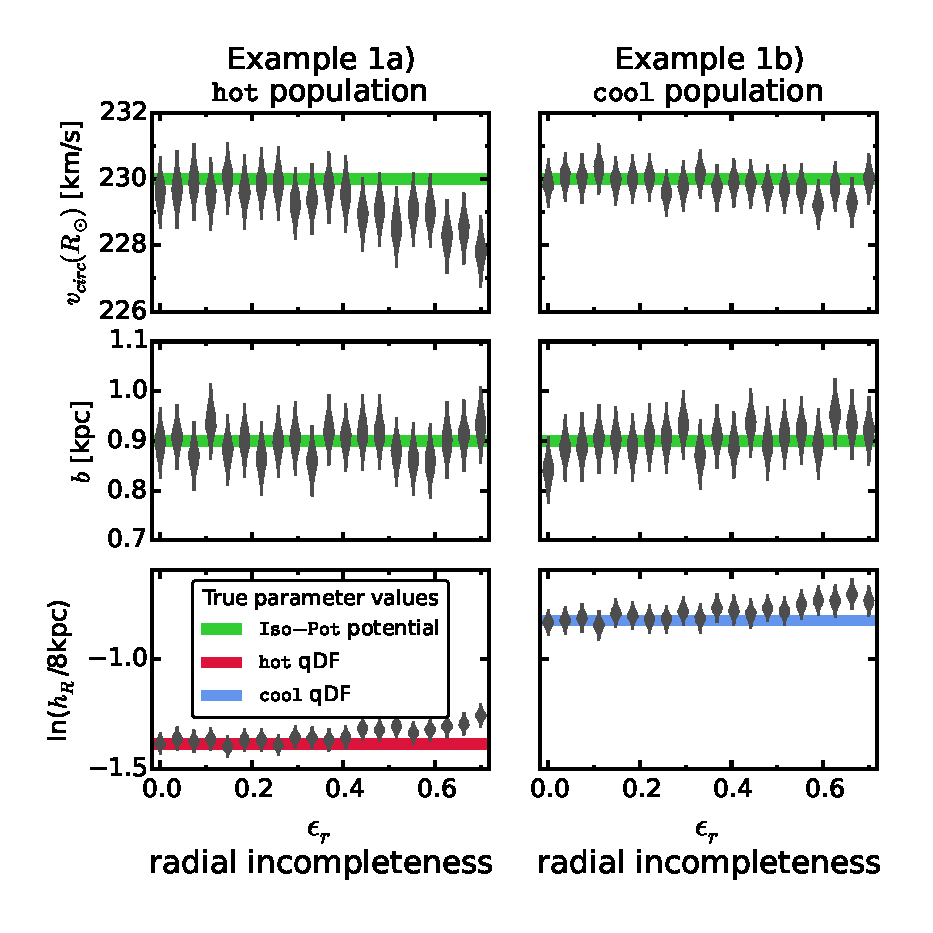
\includegraphics[width=\columnwidth]{figs/isoSphFlexIncompR_violins_2.eps}
\caption{Influence of wrong assumptions about the radial incompleteness of the data on the parameter recovery with \RM{}. Each mock data set was created with different incompleteness parameters $\epsilon_r$ (shown on the $x$-axis and illustrated in Figure \ref{fig:isoSphFlexIncompR_completeness_shapes}). (The model parameters are given as Test \ref{test:isoSphFlexIncomp} in Table \ref{tbl:tests}.) The analysis however did not know about the incompleteness and assumed that all data sets had constant completeness within the survey volume ($\epsilon_r = 0$). The violins show the full shape of the projected \pdf{}s for each model parameter, and the solid lines their true values. The \RM{} method seems to be very robust against small to intermediate deviations between the true and the assumed data incompleteness. (The qDF parameters not shown here exhibit an even better robustness than $h_R$.) \Jo{[TO DO: Jo suggested to also remove the $h_R$ panel, but I like, that one can see that it is the spatial tracer distribution that drives the little degradation of the recovery.]}} 
\label{fig:isoSphFlexIncompR_violins}
\end{figure}

%==================================================

Figure \ref{fig:isoSph_CLT} demonstrates that, given a choice of $p_\text{DF}$, a larger volume always results in tighter constraints. There is no obvious trend that a hotter or cooler population will always give better results \Wilma{[TO DO: Comment from HW: The question of whether a hotter or a colder population gives tighter constraints is an important question, but it seems buries here in a section that is dedicated to another matter, namely the question of volume ... It's OK to leave it here, but somewhere we need to say clearly: whether the population is hot or cold does not make a big and generic difference...]}; it depends on the survey volume and the model parameter in question. In Figure \ref{fig:wedFlexVol_bias_vs_SE} the wedges all have the same volume and all give results of similar precision. Minor differences (e.g., the \texttt{Iso-Pot} potential being less constrained in the wedge with large vertical but small radial extent) are a special property of the considered potential and parameters, and not a global property of the corresponding survey volume. In the case of an axisymmetric model galaxy, the extent in $\phi$ direction is not expected to matter. Overall radial extent and vertical extent seem to be equally important to constrain the potential. In addition Figure \ref{fig:wedFlexVol_bias_vs_SE} implies that for these cases volume offsets in the radial or vertical direction have at most a modest impact - even in case of the very large sample size at hand.

While it appears that the argument for significant radial and vertical extent is generic, we have not done a full exploration of all combinations of \pmodel{} and volumina.


